\begin{refsection}
\renewcommand{\thefigure}{\arabic{figure}}

\chapterTwoLines
{De como as letras formam um cidadão}
{os ritos e símbolos da Primeira República na cidade de Parelhas-RN (1928--1930)}
\label{chap:decomoasletras}

\articleAuthor
{Laísa Fernanda Santos de Farias}
{Mestranda pelo Programa de Pós-Graduação em História UFRN-CERES, professora da rede privada. ID Lattes: 4075.8724.6125.7574. ORCID: 0000-0002-2025-1259. E-mail: nandafarias07@gmail.com.}

\articleAuthor
{Sebastião Genicarlos}
{Mestre em antropologia, UFRN, professor da rede pública. ID Lattes: 7476.4847.6789.2937. ORCID: 0000-0003-3529-2851. E-mail: sebastiaosantos710@gmail.com.}

\begin{galoResumo}
    \marginpar{
        \begin{flushleft}
        \tiny \sffamily
        Como referenciar?\\\fullcite{SelfFariasAndGenicarlos2021}\mybibexclude{SelfFariasAndGenicarlos2021}, p. \pageref{chap:decomoasletras}--\pageref{chap:decomoasletrasend}, \journalPubDate{}
        \end{flushleft}
    }
    O trabalho que se apresenta, elenca enquanto temática principal a análise de como o Plano de Propaganda Contra o Analfabetismo, criado no primeiro mandato do prefeito Florêncio Luciano na cidade de Parelhas, entre os anos de 1928 a 1930, trouxe para esse município algumas noções de progresso e civilidade impostos pela Primeira República. Assim, objetivamos com este texto, explorar os desejos de desenvolvimento para a cidade pensados por Florêncio Luciano, compreender em que medida este projeto educativo promoveu novas formas de sociabilidades, e apontar como o discurso desse prefeito estava ligado a uma rede de contatos e influências que pensavam a educação também a nível estadual e nacional.  Logo, essa investigação foi possibilitada pela exploração do discurso presente no relatório de mandato, apresentado em 1930 pelo prefeito supracitado, onde foram apontadas algumas intenções e alcances trazidos pelo seu projeto educativo para os alunos parelhenses. Desta feita, com os resultados do aprofundamento da fonte aqui explorada, é perceptível elencar que a partir da leitura e reflexão dessa parte da documentação do plano, aliada à bibliografia consultada, constatamos a composição do espaço educacional parelhense alinhada à ideia de modernização e inserção de novas sociabilidades. 
\end{galoResumo}

\galoPalavrasChave{Alfabetização. Cartografia educacional. Modernização. Sertão.}

\begin{otherlanguage}{english}

\fakeChapterTwoLines
{How the letters form a citizen}
{The rites and symbols of the First Republic in the city of Parelhas-RN (1928--1930)}

\begin{galoResumo}[Abstract]
    The work that is giving to know, presents as its main theme an analysis of how the Propaganda Against Illiteracy Plan, created during the first term of mayor Florêncio Luciano in the town of Parelhas, between the years 1928 and 1930, brought to that municipality some notions of progress and civility imposed by the First Republic. Thus, with this text, we aim to explore the development wishes Florêncio Luciano thought for the town; to understand to what extent that educational project promoted new forms of sociability; and to point out how that mayor's speech was linked to a network of contacts and influences that also thought education at the level of the state and of the nation. Therefore, this investigation was made possible by the exploration of the discourse present in the mandate report, presented in 1930 by the aforementioned mayor, which pointed some intentions and the scope his educational project brought for the students from Parelhas. This time, with the results of the deepening of the source explored here, it is noticeable that from the reading and reflection of these sources combined with the consulted bibliography, we can see the constitution of the educational space of the town of Parelhas aligned with the idea of modernization and the insertion of new sociability.
\end{galoResumo}

\galoPalavrasChave[Keywords]{Literacy. Educational cartography. Modernization. Sertão.}
\end{otherlanguage}

\section{Os prelúdios do plano}

\begin{quotation}
    Se era a escola a resistência manifesta ao ímpeto modernizador, tornava-se imperioso mudá-la.

    \hfill Clarice Nunes \citeyear{Nunes1996Cultura}
\end{quotation}

Nos anos de 1920, a educação passou a ser propagandeada Brasil afora por dois grandes motivos. O primeiro deles era erradicar o analfabetismo que ainda imperava, sobretudo nos recantos mais longínquos do Rio de Janeiro, então capital da república, e dos demais centros urbanos brasileiros, gerando assim uma espécie de otimismo pedagógico\footnote{\cite[p.~261]{Nagle2009Educacao} Em seu trabalho \textit{Educação e Sociedade na Primeira República} (2009), este educador faz uma interpretação do quadro educacional brasileiro mediante o advento do estado republicano, haja vista que o do país estava vivenciando a transição de um sistema agrário comercial para um sistema industrial.}.  A escola então, como desperta a historiadora Clarice Nunes\footnote{A historiadora Clarice Nunes em seu trabalho: ``Cultura escolar, modernidade pedagógica e política educacional no espaço urbano carioca'' que se encontra na obra \textit{Missionários do progresso: médicos, engenheiros e educadores no Rio de Janeiro, 1870--1937} \citeyear{Nunes1996Cultura}, nos convida a pensar a escola enquanto um espaço de condensação simbólica dos ideais republicanos, onde os alunos seriam transformados em cidadãos da ordem e do progresso.} citada no início dessa narrativa, tornou-se um dos epicentros de formação desse novo homem agora a serviço da República.

Já o segundo ponto, se deu pelo fato de que, estando um modelo de educação estabelecido em um determinado local, o currículo escolar estava voltado para a formação de um cidadão republicano, ou seja, a prática pedagógica não estaria direcionada somente para o combate ao analfabetismo, mais do que isso, ela tinha como propósito à formação da mentalidade que se colocaria serviço da civilidade e do progresso.  

Poderíamos nos debruçar a pesquisar outros motivos que levaram a disseminação deste processo educativo, porém, pensamos que os dois ensejos supracitados, traduzem as urgências de uma época em que o país estava saindo de um modelo imperial e adentrando um período em que importava para os líderes republicanos, formar cidadãos que estivessem em consonância e adequados às mudanças sociais e urbanas que advinham da Europa. Esses ideais: 

\begin{quotation}
    Eram inspirados no modelo puritano, ascético e europeu ganharam corpo nas reformas sanitárias, pedagógicas e arquitetônicas deste século. Esses valores foram aglutinados em formulações filosóficas e científicas que procuravam ter junto a sociedade um efeito moral, normatizador. A palavra de ordem é sintonizar-se com a Europa, ou melhor, ``civilizar-se'' o mais rápido possível, de modo que o país pudesse, o quanto antes, competir com no mercado internacional \cite[p.~26]{HerschmannAndPereira1994Invencao}.
\end{quotation}

Após os republicanos assumirem o poder, o direcionamento principal era o de instruir a população a partir das diretrizes de transformações ocorridas na Europa, no que se referiam ao cotidiano, à dinâmica urbana com as transformações das cidades, bem como na adaptação do homem para lidar com as novas manifestações industriais e econômicas ocorridas naquele momento\footnote{A chamada Revolução Científico-Tecnológica que ocorreu em meados do século XIX, mas atingindo sua hegemonia no final de 1870, impulsionou a produção de novos potenciais energéticos, novas formas de metalurgia e processos químicos, bem como a produção de artifícios que facilitaram a comunicação, o transporte e o cotidiano das pessoas. Essa discussão está em: \fullcite{Sevcenko1998Preludio}.}. ``Urgia, `civilizar' o país, modernizá-lo, espelhar as potências industriais e democratizadas, e inseri-lo compulsória e firmemente no trânsito de capitais, produtos e populações liberados pelo hemisfério norte''. \cite[p.~134]{Marins1998Habitacao}.

Por meio disso, justificamos que o interesse em trabalhar essa temática, relaciona-se ao fato de que, se havia um projeto educativo em Parelhas, recanto sertanejo do Rio Grande do Norte, que estava ligado a uma perspectiva de formação do povo brasileiro, compreende-se que podemos pensar o Sertão envolto nas suas mais diversas antinomias, enquanto um projeto de modernidade.  

A educação vinculada à instrução primária e nos modelos escolares que passaram a se expandir pelo Brasil, funcionou enquanto uma mola mestre na retirada do atraso e das heranças coloniais e imperiais ainda presentes neste novo momento, o que no sertão do Seridó não seria diferente.  

Na espacialidade aqui tratada, Manoel Dantas, por exemplo, que se destacou no movimento republicano no sertão do Seridó e no estado do Rio Grande do Norte, trouxe de sua formação acadêmica no Recife\footnote{Segundo \textcite{Macedo2005}, ainda em sua obra \textit{A Penúltima Versão do Seridó: uma história do regionalismo seridoense}, a faculdade do Recife era um verdadeiro celeiro das ideias progressistas e as teorias politicas e ideológicas do pensamento republicano. Logo, os seridoenses estudantes dos cursos de Direito ou Medicina acabam trazendo todo esse arcabouço ideológico alinhado ao pensamento e objetivos da Primeira República para o Seridó.} os ideários e os debates ideológicos acerca do progresso e civilidade em busca de um novo homem para o Seridó.

\begin{quotation}
    Um tempo mais acelerado, impulsionado por novos potenciais energéticos e tecnológicos, em que a exigência de acertar os ponteiros brasileiros com o relógio global suscitou a hegemonia de discursos técnicos, confiantes em representar a vitória inelutável do progresso e por isso dispostos a fazer valer a modernização a ``qualquer custo'' \cite[p.~27]{Sevcenko1998Preludio}.
\end{quotation}

Nos ponteiros do relógio de educadores como Manuel Dantas\footnote{Manuel Dantas, caicoense, nasceu em 26 de abril de 1867 e faleceu em Natal em 15 de unho de 1924. Foi advogado e juiz, devendo sua formação a faculdade de Ciências Jurídicas e Sociais pela Faculdade de Direito do Recife no ano de 1890 onde acabou sendo influenciado pelos ideais republicanos e trazendo todo este arcabouço teórico e cientifico para o pensamento educacional norte rio-grandense durante a sua atuação enquanto diretor geral de educação, pensando ainda nas mudanças que esse novo pensar poderia trazer no tocante a mudança ou a adequação do homem sertanejo ao modelo republicano.}, Diretor Geral de Instrução Pública, na década de 1920, e que escreveu diversos estudos e ponderações\footnote{Além de escrever desde o final do século XIX para o jornal O Povo, periódico esse que já tinha um viés republicano, no âmbito educacional, Manuel Dantas se destaca por suas publicações nas revistas do Instituto Histórico e Geográfico do Rio Grande do Norte, mais precisamente na Revista Pedagógium onde publicou artigos como, Escolas Rudimentares, que será aprofundado mais adiante.} tanto sobre a organização do ensino na capital do estado, como também acerca dos processos de interiorização da educação via Escolas Rudimentares, o tempo do homem seridoense deveria ser o da adequação aos elementos que a República estava buscando em relação ao desenvolvimento urbano e antropológico do sertão do Seridó, com sustentação em esfera nacional.  

Para este educador, o comportamento letárgico do homem sertanejo aparecia como um empecilho ao desenvolvimento do interior. A necessidade de transformação deste personagem, apesar da importância dada à tradição, era necessária. Com isso, a este homem era dada a tarefa de acompanhar as mudanças trazidas pela República, se adequando aos seus direitos e deveres de cidadão, não tendo um comportamento pautado somente em suas tradições, e constituindo-se assim enquanto um ser humano pensante e articulador dos desejos progressistas daquele período.  

Prontamente, a cultura latente do sertanejo pautada na memória e nas tradições, acabaria atrapalhando o desenvolvimento e acabaria fossilizando-o no passado. Com isso, o aspecto ruralizado do sertanejo, apesar de importante como reconhecia Manoel Dantas, precisava ser readequado pela lei do progresso. Desse modo, podemos entender que:

\begin{quotation}
    O Brasil da Primeira República era também o país dividido entre os ``políticos bacharéis'' e os ``homens de ação''. A ruptura com o atraso brasileiro significava, para muitos desses homens, a reorganização, em bases racionais e técnicas, do trabalho agrícola, da fixação do homem rural, dos instrumentos e agências de produção. Embora majoritariamente rural, o Brasil já tomava contato com a aceleração urbana, e, simultaneamente, com a precariedade do investimento em educação --- fonte, àquela altura, primordial ao enfretamento da necessária qualificação para o trabalho. \cite[p.~320]{Bomeny2014Educacao}.
\end{quotation}

Partindo desse pressuposto, os arranjos e mudanças sociais a partir da disseminação de valores civis que tinham como intuito principal homogeneizar as referências sociais do país em um discurso voltado para o progresso e civilidade, também correspondiam ao momento em que o desenvolvimento intelectual das elites seridoenses estava em franca ascensão por meio do contato com a Faculdade de Direito do Recife que se encontrava envolta nas discussões calorosas acerca da propaganda republicana.  

Esse debate não passou despercebido pela socióloga Nísia Trindade Lima \citeyear{Lima2013Sertao} que, ao pesquisar acerca dos intelectuais brasileiros que pensaram o sertão, não deixou de elencar o papel da República neste processo. Segundo a autora:

\begin{quotation}
    Os primeiros anos da República foram palco de um expressivo movimento de valorização do sertão, seja enquanto espaço a ser incorporado ao esforço civilizatório das elites políticas do país, seja como referência da autenticidade nacional. \cite[p.~114]{Lima2013Sertao}.
\end{quotation}

Pensando a partir dessa discussão e da necessidade de Manuel Dantas em enquadrar o homem sertanejo a um projeto progressista, percebemos que as contrariedades entre sertão e litoral não eram incongruentes, mas sim passíveis de harmonização. E, neste caso, a educação converteu-se em um recurso que poderia incorporar o interior a um projeto de Brasil. 

Por meio disso, as mensagens com ideias moralizantes e que seriam a partir de agora amplamente propagadas pelas escolas primárias, e no caso do sertão, pelas Escolas Rudimentares, continham a existência de diversas alegorias patrióticas e ufanistas que incentivavam a modelação desse homem sertanejo. 

Nas engrenagens deste processo, a República pretendia criar um modelo de cidadão civilizado, entendedor da ordem vigente e que, juntamente com seu governo, pudesse construir um país sobre a esteira do progresso e do desenvolvimento urbano, higienista e instrucional. Os vislumbres desse ideário estavam pautados na concepção de que seria encaminhada ``à educação a função de agente transformadora dos súditos brasileiros em cidadãos republicanos'' \cite[p.~81]{Stamatto2005Escola}.

Ao escolhermos elencar a tríade de desenvolvimento do país anteriormente citada que se distribuiu em uma organização urbana, na higiene e educação, convocamos em nossos estudos Herschmann e Pereira (1994), no que concerne a problematizar as transformações das cidades republicanas por meio dos projetos de organização dos espaços citadinos, em seu sistema de saúde ponderando nos cuidados com o corpo, e ainda a expansão da educação na ideia da ``conformando mentalidades''\footnote{O uso do termo \textit{conformando mentalidades}, discutido por Herschmann e Pereira \citeyear{HerschmannAndPereira1994Invencao} no trabalho ``A invenção do Brasil Moderno: medicina, educação e engenharia nos anos 20--30'', compreende-se os ideais republicanos como progresso, civilidade, e novos comportamentos que passaram a ser inculcados nos currículos escolares com o intuito de formar um cidadão adequado aos trâmites deste novo período.}.

No caso da última característica desse tripé de desenvolvimento de um Brasil moderno, em que se sucedem os anos de 1920, a educação, objeto de análise desta narrativa, vem sendo pensada enquanto uma vertente da chegada da modernidade em Parelhas-RN no final do período da Primeira República. Modernidade esta que, torna-se uma prática educativa quando da aplicação dos conteúdos em sala de aula por meio de símbolos como a Bandeira, o Hino, e a seleção de conteúdos para formar cidadãos que zelassem por seu país, e que alimentando tal zelo, tivessem uma nova perspectiva de desenvolvimento para o mesmo.

Partindo deste pressuposto, a narrativa em questão tem como principal objetivo, apresentar como o Plano de Propaganda Contra o Analfabetismo, evento ocorrido em Parelhas-RN, no Sertão do Seridó, acompanhou os discursos nacionais e promoveu uma educação pautada na disciplinarização de mentes e formação de cidadãos que passassem a seguir os trâmites impostos pelos governos republicanos. Logo, usamos como material para exemplificar este processo, o relatório de mandato do prefeito Florêncio Luciano, articulador do plano, quando relatou uma das festas cívicas realizadas na cidade, sendo esta elaborada pelos professores e alunos deste projeto educacional. 

Tudo isso será discutido por meio de um corpo investigativo que problematiza os aspectos da Modernização a partir de Fredric Jameson \citeyear{Jameson2005Modernidade}, David Harvey \citeyear{Harvey2002Condicao} e o próprio Marshal Berman \citeyear{Berman1986Tudo} que forneceu o suporte teórico para investigar como na prática, se incorporaram as mudanças propostas por meio do Plano de Propaganda Contra o Analfabetismo no espaço da cidade de Parelhas. Além dos debates que envolvem as mudanças trazidas pela República a partir de historiadores como José Murilo de Carvalho \citeyear{Carvalho1990Formacao} e Nicolau Sevcenko \citeyear{Sevcenko1998Preludio}, Herschmann e Pereira \citeyear{HerschmannAndPereira1994Invencao}, Nísia Trindade Lima \citeyear{Lima2013Sertao}, além de Veiga e Fonseca \citeyear{VeigaAndFonceca2003Historia}, no que concernem as abordagens simbólicas da formação do homem no período em discussão.

Sem mais, teríamos aspectos de modernização sendo aplicados não só numa perspectiva física, ou seja, na construção de escolas, no uso do telégrafo, instalação e ampliação da rede elétrica, assim como nos trâmites simbólicos distribuídos em textos trabalhados em sala de aula, o uso do hino, organização das turmas, fardamento e desfiles cívicos que passaram a fazer parte das aulas e que moldavam os alunos na busca pela formação de um novo homem sertanejo.

\section{A república nas entrelinhas do plano}

O Plano de Propaganda Contra ao Analfabetismo criado e articulado por Florêncio Luciano\footnote{Segundo o pesquisador local Tertuliano Pereira em seu folheto mensal; \textbf{Memórias de Parelhas: resumo de Vida e Obras}, impresso pela gráfica Vilar em junho de 2018, Florêncio Luciano nasceu na comunidade rural Boa Vista dos Lucianos, município de Parelhas, no dia 2 de novembro de 1894, era filho do agricultor e artífice de fogueteiro José Luciano e entrou na vida política em 1927 após o desligamento da cidade de Parelhas de Jardim de Seridó. \cite[p.~2]{Pereira2018Memorias}.}, prefeito que assumiu a administração municipal entre os anos de 1928 até 1930, passou a investir maciçamente na educação parelhense criando desde as Escolas Rudimentares\footnote{Escolas Rudimentares refere-se ao investimento a um modelo escolar simples que tanto poderia ser instalada em espaços já existentes de uma cidade, como também na construção de alguns prédios. Neste local, o curso ofertado seria uma alfabetização inicial com leitura, escrita, matemática, além das noções de conhecimentos gerais e instrução cívica, constituindo assim um curso primário.} e consequentemente a isso fazendo uma série de contratação de professores. Para tanto, o prefeito ainda investiu na época em um curso preparatório para os docentes, e montou uma teia de vistoria pedagógica que tinha como incumbência principal além de fazer recenseamentos, mas também fiscalizar os andamentos das aulas, bem como a assiduidade dos alunos\footnote{Para ter um detalhamento do que foi o Plano de Propaganda Contra o Analfabetismo, acesse o trabalho: Florêncio Luciano e o Plano de Propaganda Contra o analfabetismo: modernização pela educação no Sertão do Seridó Potiguar (1928--1929). Disponível em https://periodicos.ufrn.br/histela/article/view/19500, acesso em: 15 de abril de 2021.}.

Este plano consistiu em eliminar o analfabetismo presente no município de Parelhas e criou uma série de artifícios para que os seus objetivos fossem concretizados. Desta forma, podemos dividir em três categorias a estrutura utilizada por esse projeto educativo no desenrolar do seu processo, são elas: as criações das Comissões Urbana, Rural e Central contra o analfabetismo que teve um importante papel para demarcar os sujeitos que foram alfabetizados; a criação das escolas e contratação de professores enquanto uma logística do plano propriamente dito assim como as atividades pedagógicas realizadas; e as instituições que passaram a fiscalizar o desenvolvimento desse plano. 

No início de 1930 o então prefeito de Parelhas, Florêncio Luciano, faz um balanço do ano anterior do seu mandato. Abordando questões que foram ampliadas naquele período desde a arborização da cidade, sua zona agrícola, instrução pública, obras públicas, rodovias e entre outros aspectos do desenvolvimento da respectiva urbe, esse gestor, conseguiu expressar em seu relato toda a satisfação de ter dado incentivo inicial para o progresso de uma antiga vila que entrava no rol dos municípios do estado do Rio Grande do Norte. Ao iniciar seu testemunho, é possível perceber essas questões, vejamos: 

\begin{quotation}
    Para levar avante as idèas germinadas no meu cérebro, as quaes eram promover o progresso dentro das esferas das nossas possibilidades, necessário foi promover o alevantamento das nossas rendas, a arrecação das mesmas, porque entendo ser a base essencial para promoverem-se os melhoramentos públicos pela evolução hodierna do nosso povo. (RELATÓRIO, 1929, n.p.).
\end{quotation}

Diante do que foi abordado, Florêncio Luciano deixou clara a sua afeição para o progresso da cidade, montando já para a efetivação deste, toda uma logística de arrecadação para promover os melhoramentos que, segundo ele, faziam parte da evolução do povo parelhense. Questão essa que se relaciona com as propostas sugeridas pelos governos republicanos e que o historiador José Murilo de Carvalho em sua obra \textit{A formação das Almas: o imaginário da República no Brasil} (1990) irá discutir no tocante às ideologias propagadas entre aqueles que estariam a frente de todo e qualquer processo político. Com isso:

\begin{quotation}
    Os temas do interesse do indivíduo e de grupos, da nação, da cidadania, encarnados na ideia de república, estavam no centro das preocupações dos construtores da República brasileira. Como país exportador de matérias-primas e importador de ideias instituições, os modelos de república existentes na Europa e na América, especialmente nos Estados Unidos e na França, serviriam de referência constante aos brasileiros. \cite[p.~18]{Carvalho1990Formacao}.
\end{quotation}

Com isso, é perceptível a relação das ideias aguçadas por Florêncio Luciano acerca do progresso parelhense com as vertentes do desenvolvimento que imperavam no Brasil naquele período. A preocupação dos líderes políticos nacionais, como também do líder em questão era disseminar esses ideais pela população. E, nisso, a educação se tornou peça fundamental para moldar principalmente os analfabetos para buscar junto as instituições do estado, uma espécie de corrente do desenvolvimento e progresso deste país. Desta feita, tratava-se de montar uma rede de ensino no país que desse conta da formação do caráter do cidadão, a sua moralidade, além dos sentimentos patrióticos enquanto a constituição de uma identidade nacional

Ao falar especificamente do seu projeto educativo nesse relatório, o gestor deixou clara a sua satisfação para com as conquistas conseguidas por meio do seu plano até aquele momento, fazendo com que a Propaganda Contra o Analfabetismo construísse novas atribuições na vida dos seus alunos. Com isso, este político acenou:

\begin{quotation}
    Com a propaganda contra o analfabetismo, que levei avante no município, contando com a colaboração do povo em geral de minha terra, consegui elevar a matrícula nas escolas estaduaes municipaes para mais de 600 alumnos. [\dots] Instruir é educar, e sem educação não podemos ingressar no caminho da civilização, pois é um dos requisitos indispensáveis ao homem civilizado --- saber ler e escrever (LUCIANO, 1929, n.p).
\end{quotation}

Diante disso, entende-se que o prefeito trouxe para a sua discussão a ideia de civilização, de instrução e de consequente a educação enquanto uma saída para um novo modelo de sociedade. Para a república, o analfabetismo da imensa população poderia representar um impedimento à construção de uma nação moderna e civilizada que deveria ser pensada não só pelas instituições governamentais como também pelo próprio povo, responsável pela continuidade deste processo.  

As perspectivas alimentadas e realizadas pelo prefeito correspondiam a um retrato de um país delineado ao longo dos anos 20 e 30, mas que já vinham surgindo em um Brasil de fins do século XIX a partir dos valores e modelos de sociedade que uma elite dominante queria empregar. 

Ao deixar claro que a organização citadina precisava de ordem, e que sem ela não haveria progresso e evolução, Florêncio Luciano estava em sintonia com um projeto de Brasil que já vinha se esquematizando nas grandes capitais. Esses ideais:

\begin{quotation}
    Eram inspirados no modelo puritano, ascético e europeu ganharam corpo nas reformas sanitárias, pedagógicas e arquitetônicas deste século. Esses valores foram aglutinados em formulações filosóficas e científicas que procuravam ter junto a sociedade um efeito moral, normatizador. A palavra de ordem é sintonizar-se com a Europa, ou melhor, ``civilizar-se'' o mais rápido possível, de modo que o país pudesse, o quanto antes, competir com no mercado internacional \cite[p.~26]{HerschmannAndPereira1994Invencao}.
\end{quotation}

Desse modo, é perceptível a relação das ideias aguçadas por Florêncio Luciano acerca do progresso parelhense com as vertentes do desenvolvimento que imperavam no Brasil naquele período. Em outro momento neste mesmo relatório, o prefeito nos descreve acerca da realização de uma atividade no dia 15 de novembro de 1929, em que o desperta para os resultados que já tinha conseguido com seu projeto ao longo do mesmo ano. Neste documento, este personagem relata a realização de uma festa cívica escolar alusiva ao dia 15 de novembro:

\begin{quotation}
    Tive a idéa, e levei a efeito com o fim exclusivamente de incentivar cada vez mais o ensino no município, promover uma festa cívica-escolar no dia 15 de Novembro passado, data da proclamação da Republica, reunindo nesta cidade, 505 alumnos, devidamente uniformizados. [\dots] Assim, na manhã daquele dia, Parelhas assistiu um dos mais soberbos espetaculos, vendo desfilar em passeata cívica, uniformizada e em ordem a mocidade esperançosa de nossa terra, cuja festividade deixou um marco na história de Parelhas (LUCIANO, 1929, n.p).
\end{quotation}

Ao promover uma festa alusiva referente aos 15 de novembro, o prefeito buscou antes de tudo elementos que faziam referência à legitimação dos regimes políticos que tinham como base trazer aspectos do moderno. Neste sentido, a República foi incisiva ao expandir símbolos, ritos e mitos que conseguissem fazer com que a população obtivesse uma concepção de país e consequentemente de progresso, de busca de adiantamento, civilidade. Com isso, ao trazermos o exemplo da comemoração do dia 15 de novembro em 1929, pensamos que a imagem consegue nos evocar como este processo de disciplinarização de mentes e corpos estava acorrendo.

\begin{figure}[ht]%
    \centering%
    \caption{Registro fotográfico da turma do professor Simião de Oliveira Mello em 1929.}%
    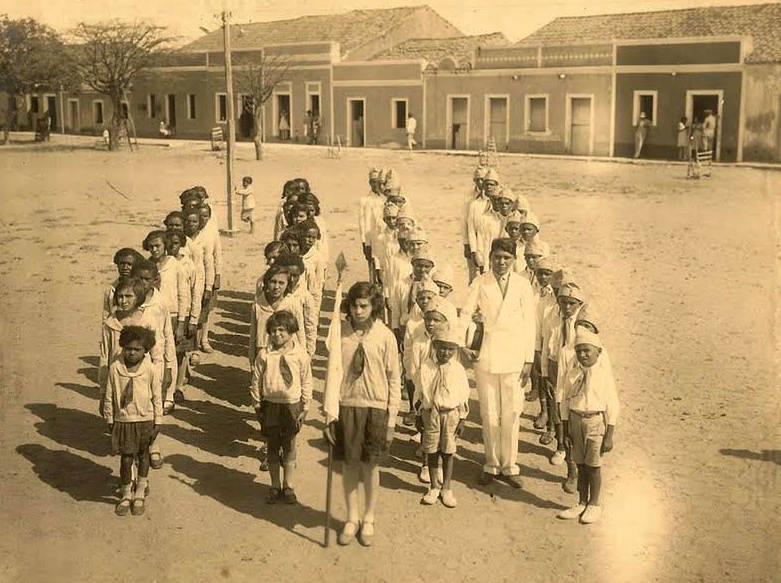
\includegraphics[width=.85\textwidth]{articles/04-de-como-as-letras-fo/01-turma-professor.jpg}%
    \caption*{Fonte: Arquivo particular do historiador local Tertuliano Pereira\\
    Autor: Laísa Fernanda Santos de Farias utilizando do acervo do historiador local Tertuliano Pereira.}%
    \label{fig:turmaProfessor}%
\end{figure}%

Observemos a fotografia na página \pageref{fig:turmaProfessor}. Nela o relato do prefeito Florêncio Luciano se confirma. Nos corpos, posturas e simbologias como o uso do fardamento, além do próprio uso da bandeira, simbolizando o respeito e admiração pela República, fica clara a inscrição a expansão do projeto do referido prefeito. Acima, o progresso e o desenvolvimento, abaixo, a terra batida e a pouca estrutura. De um lado, professor e crianças com outra perspectiva de cidade, ao fundo, poucas casas e um cenário urbano que ainda carrega aspectos de um ambiente rural, mas que naquele momento estava presenciando os primeiros signos da modernidade através da Educação.  

O resultado de uma modernidade baseada na construção ou manutenção de uma escola acaba depositando na cidade uma série de artifícios. O Plano de Propaganda Contra o Analfabetismo também acabou promovendo em Parelhas a chegada de uma série de outros recursos que também facilitaria sua existência. A luz elétrica representava para uma vila que acabava de se tornar cidade um avanço, pensada também para melhorar o acesso e permanência dos alunos deste plano nas escolas parelhenses. Neste sentido, ``o conceito de modernidade, característico deste conjunto de intervenções, sintetiza essas aspirações'' \cite[p.~68]{Dias2012Laranjas}.

Mas, eram nas salas de aulas que este processo ocorria com mais intensidade. Para além do registro já apresentado e o próprio relato de Florêncio Luciano, apresentamos ainda o roteiro\footnote{Este relato encontra-se no documento: Papéis Diversos Referentes à Instrução Pública e festa de 15 de novembro de 1929, na caixa Receitas e Despesas de 1929 a 1930.} de uma festa alusiva ao dia 7 de Setembro também do ano de 1929 que aconteceria no centro da cidade. Neste sentido, dividido em quinze partes o itinerário de apresentação construído trazia desde declamações de poesia, apresentações de pequenas peças de teatro e histórias diversas, além de canções. Porém, o que nos chama atenção são as apresentações que diziam respeito ao:

\begin{quotation}
    \noindent\rule{.87\textwidth}{0.4pt}
    
    \begin{center}
                    Programma da festa 7 de setembro. 1929. \\
                         1ª Parte Cívica. 7 horas
    \end{center}

    \renewcommand{\labelenumi}{\Roman{enumi}}
    \begin{enumerate}
        \item Hasteamento da Bandeira e Hynno a Bandeira; 
        \item Preleção sobre a data, pelos professores e suas classes respectivas; 
        \item Recitativas de poesias patroticas.
    \end{enumerate}

    \begin{center}
                        II Parte. Recreativa. 19 ½ horas\\
                         No edifício do Cinema piranga. 
    \end{center}

    \begin{enumerate}
        \item Belezzas do Brasil --- Dialogo --- pelas alumnas Maria Alice e Guiomar Oliveira.
    \end{enumerate}

    \noindent\rule{.87\textwidth}{0.4pt}
\end{quotation}

Neste trecho da documentação, encontramos a divisão de apresentações de cunho cívico, onde a intenção era levar os alunos a declamarem os símbolos patrióticos zelados pela República, e ainda uma parte mais recreativa como intitula o próprio documento, mas que mesmo assim não deixaria de enfatizar os signos nacionais por meio das belezas do Brasil. Logo, percebemos que a conformação de mentalidades já citadas acima em \textcite{HerschmannAndPereira1994Invencao}, nos ajuda a refletir como estas práticas educativas traduzem uma época, e ainda demonstram uma necessidade para que o homem do republicano, ao contrário dos súditos do império, tivessem conhecimento da pátria que pertenciam e soubessem construí-la a começar por sua consideração.  

Estudiosos como Fredric Jameson \citeyear{Jameson2005Modernidade}, David Harvey \citeyear{Harvey2002Condicao} e o próprio Marshal Berman \citeyear{Berman1986Tudo} tem dado suporte teórico para pensar a modernidade enquanto um fenômeno social e tecnológico, o que nos ajudou a compreender neste trabalho, o espaço parelhense e as mudanças trazidas por meio do Plano ao próprio sertão seridoense.

Harvey, por exemplo, destaca em sua obra Condição Pós-Moderna a seguinte questão:

\begin{quotation}
    A modernidade, por conseguinte, não apenas envolve uma implacável ruptura com todas e quaisquer condições históricas precedentes, como é caracterizada por um interminável processo de rupturas e fragmentações internas inerentes. \cite[p.~22]{Harvey2002Condicao}.
\end{quotation}

Ao ligarmos essa condição defendida por Harvey ao Plano de Propaganda Contra o Analfabetismo, abre-se a perspectiva para compreender o Sertão e suas educabilidades enquanto a ruptura de um processo de atraso educacional alertado pelo modelo de governo republicano e que seria resolvido por meio da distribuição ou da fragmentação dessa ideia em diversas localidades, como a própria cidade de Parelhas.  

O Sertão aqui investigado por meio da educabilidade remete-se a um lugar contemporâneo e consequentemente urbano, já que o projeto aqui elaborado pensou intuitivamente no desenvolvimento da sua Zona Rural, bem como da própria Urbe.  

Em Fredric Jameson a discussão concentra-se em pensar esse Sertão aqui representado enquanto um espaço de produção e mobilidade. Para este autor, em sua obra \textit{Modernidade Singular: Ensaio sobre a ontologia do presente}, destaca a seguinte questão:

\begin{quotation}
    O Tropo da modernidade pode ser considerado naquele sentido auto-referente, se não performativo, já que sua aparição sinaliza a emergência um novo tipo de figura, uma quebra decisiva com a forma prévia de um novo tipo de figurativismo, e é nessa medida um sinal da própria existência, um significante que indica a si próprio e cuja forma é o seu próprio conteúdo. \cite[p.~45]{Jameson2005Modernidade}.
\end{quotation}

Diante do que foi exposto é necessário explicar inicialmente que, aproprian\-do-se do discurso de Jameson, este \textit{tropo} presente no Plano era é o avanço da cidade por meio da alfabetização dos seus cidadãos. Porém, outros signos da modernidade também são encontrados no tocante a própria manutenção das escolas nesse período. 

A instalação da luz elétrica, por exemplo, faz parte deste processo, pois a educação, neste contexto, notifica uma série de outros meios que até então não eram vistos no Sertão. Com isso, pode-se citar o exemplo do documento referente à instalação da luz elétrica nos salões do Barão do Rio Branco. Temos a seguinte abordagem:

\begin{quotation}
    Os abaixo assinados, Silva e Dantas, vêm com o presente pedir a V.S. se digne de mandar pagar aos mesmos a importância de 106\$900...?, proveniente de material e mão de obra de uma instalação de luz elétrica nos salões do grupo Escolar ``Barão do Rio Branco'' e feita pelos suplicantes, conforme documento junto. Nestes termos, P. defirimento\footnote{Abaixo assinado feito para o Prefeito Florêncio Luciano liberasse verba para a instalação da luz elétrica no grupo escolar Barão do Rio Branco. Informação encontrada no documento referente à Receita de 1929 encontrado na caixa: Receitas de 1929, no arquivo da prefeitura municipal de Parelhas.}. (RECEITAS, 1929, n.p).
\end{quotation}

A partir do relato documental acima, fica visível a problematização do autor Fredric Jameson ao identificar o que é o tropo da modernidade. A forma do próprio conteúdo identifica a emergência de um novo tipo de figura, ou seja, de um novo tipo de característica dada a um determinado lugar. Ao concatenar a sua problematização com a manutenção do grupo escolar acima cita, temos um novo tipo de performance para ler o Sertão.  

Nesta oportunidade, a cidade de Parelhas se constitui enquanto um lócus de experiência de modernidade. Esses equipamentos expressavam novas formas técnicas, de avanços científicos, além de empregar outra cadência de vida, neste caso, participativa e facilitadora da rotina da educação.  

Convoca-se ainda para entender a modernidade enquanto presença no Sertão, o Filósofo Marshall Berman em seu trabalho Tudo que é sólido se desmancha no ar. Compreendendo que a modernidade atrelada à vida urbana só é possível quando a cidade se torna o próprio instrumento de argumentação.  

Prontamente, são experiências de vidas e espaços que são compartilhados por todos e dessas experiências surge uma amplitude de visões e ideias que visam tornar as pessoas sujeitos e objetos desse processo. Com isso, \textit{``ser moderno é encontrar-se em um ambiente que promete aventura, poder, alegria, crescimento, autotransformação e transformação das coisas em redor --- mas ao mesmo tempo ameaça destruir tudo o que temos, tudo o que sabemos, tudo o que somos.''} \cite[p.~15]{Berman1986Tudo}.

\section{Algumas conclusões}

Chegando ao final desta discussão, é importante deixar claro que este escrito faz parte de um projeto dissertativo que ainda está em construção e que ainda não consegue elencar resultados assertivos sobre o Plano de Propaganda Contra o Analfabetismo. Porém, por meio das leituras aqui realizadas, temos a primeira conclusão sobre o desenrolar deste projeto. A cidade e seus espaços que geralmente tem seu processo modernizador atrelado ao desenvolvimento dos projetos de urbanização, aqui vem sendo investigado e repensado por meio da educação, ela é quem traz esse processo modernizador.  

Logo, o discurso do prefeito Florêncio Luciano, expresso em seu Relatório de mandato de 1930, que discorria sobre progresso, civilidade e desenvolvimento, nos traz uma das possibilidades do crescimento de Parelhas por meio também da educação, e não só pelas reformas urbanas características nos anos 20. 

Com isso, o Plano de Propaganda Contra o Analfabetismo elaborado por Florêncio Luciano e seus condescendentes torna-se um gesto de contestação, refutação e problematização aos discursos impregnados sobre o Sertão enquanto um lugar atrasado e obsoleto onde o aspecto rural prevalecesse em relação ao urbano, questão essa que é completamente errônea se pensarmos no desenvolvimento das cidades nordestinas que aumentam após a década de 70, mas que já privilegiavam seu desenvolvimento por projetos como o de Florêncio Luciano ainda no início do século XX.

\section{Considerações finais}

Quando se fala em experiência educativa, não interessa aqui uma memória individual daquilo que foi vivido, mas sim, de um conjunto de metodologias que alcançou um vultoso número de pessoas. A educação não é um processo singular, mas sim pensado em abarcar um todo, logo a alfabetização de uma pessoa não tiraria o atraso instrucional de uma população e nem tampouco a transformaria em um modelo de sociedade voltada para o progresso e civilidade, só se mesma fosse pensada numa coletividade como assim o fez o Plano de Propaganda Contra o Analfabetismo. 

Chegando ao final desta narrativa, acreditamos que ao citar uma pequena parte de uma vasta documentação sobre o Plano de Propaganda Contra o Analfabetismo, esperamos ter conseguido mostrar ao leitor como em Parelhas-RN se constituiu uma experiência educativa. Logo, são experiências de vidas e alfabetização que são compartilhados por todos e desses experimentos, surge uma amplitude de visões e ideias que visam tornar as pessoas sujeitos e objetos desse processo que foi a educação na primeira República.  

O Plano de Propaganda Contra o Analfabetismo acabou se efetivando e se perpetuando nas instalações de prédios escolares, nos materiais distribuídos aos alunos, nos recenseamentos para matricular os educandos ou ainda nos próprios desfiles cívicos que acabaram sendo internalizados nas reminiscências tanto daqueles que viveram a época, quanto daqueles que cresceram sabendo que seus pais ou avós foram alfabetizados por meio dos objetivos deste plano ou ainda sabendo das histórias das professoras que alfabetizou algum membro de sua família. 

Ademais, no período em que o sobredito plano esteve em vigor, o instrumental arregimentado para o seu funcionamento teve como resultado indireto um conhecimento mais nítido da realidade populacional do jovem município parelhense. Uma vez que, além da questão demográfica, com atenção especial para os jovens, público alvo do intento educador, houve a mobilização e o emprego dos poucos letrados aí residentes e a modernidade marcou indelevelmente sua presença por meio do telégrafo, da eletricidade e da própria construção de prédios escolares, símbolo maior da vida moderna, tanto no espaço urbano, quanto na zona rural. Temos então, a produção de uma cultura material que faz referência um projeto de desenvolvimento da cidade pensado inicialmente por seu viés educativo.

\printbibliography[heading=subbibliography,notcategory=fullcited]

\hfill Recebido em 5 abr. 2021.

\hfill Aprovado em 18 abr. 2021.

\label{chap:decomoasletrasend}

\end{refsection}
